\chapter{Registro de asistencia}

La validación de GAMMA incluyó dos sesiones formales con el equipo: una capacitación inicial al arranque del período de uso, y una sesión de seguimiento de resultados. El Cuadro \ref{tab:asistencia} resume la asistencia registrada en ambas, agrupada por rol para preservar la confidencialidad de las personas involucradas.

\begin{table}[!htb]
\centering
\caption{Asistencia registrada por rol en las sesiones de capacitación y seguimiento}
\label{tab:asistencia}
\begin{tabular}{lrr}
\toprule
\textbf{Rol} & \textbf{Capacitación inicial (18 jun 2026)} & \textbf{Seguimiento (16 jul 2026)} \\
\midrule
Equipo UVG - MBIA & 3 & 3 \\
Jefatura & 1 & 1 \\
Coordinación & 1 & 1 \\
Gestores & 5 & 5 \\
\midrule
\textbf{Total} & \textbf{10} & \textbf{10} \\
\bottomrule
\end{tabular}

\end{table}

\chapter{Instrumento y respuestas de la encuesta de satisfacción}

La encuesta se aplicó mediante un formulario con lógica de ramificación según el rol y la experiencia de uso del respondiente. Se obtuvieron 5 respuestas: 3 de gestores que utilizaron GAMMA activamente, y 2 de jefatura y coordinación del área.

\section*{Respuestas de gestores (n=3)}

\begin{table}[!htb]
\centering
\small
\caption{Respuestas de los gestores que utilizaron GAMMA}
\label{tab:encuesta-gestores}
\begin{tabular}{p{5.5cm}ccc}
\toprule
\textbf{Pregunta} & \textbf{Gestor 1} & \textbf{Gestor 2} & \textbf{Gestor 3} \\
\midrule
Facilidad de uso (1--5) & 5 & 5 & 5 \\
Utilidad de la sugerencia de descripción (1--5) & 5 & 4 & 4 \\
Precisión de la clasificación sugerida (1--5) & 4 & 3 & 4 \\
Reducción de tiempo percibida (1--5) & 5 & 3 & 4 \\
Satisfacción general (1--5) & 5 & 4 & 4 \\
¿Recomendaría GAMMA? (1--5) & 5 & 4 & 5 \\
\bottomrule
\end{tabular}
\end{table}

\textbf{Módulos utilizados:} Gestor 1 usó los tres módulos y la exportación a Excel; Gestor 2 usó normalización, duplicados y clasificación; Gestor 3 usó únicamente normalización.

\textbf{Parte más valiosa:} los tres gestores coincidieron en señalar la detección de duplicados; Gestor 1 y Gestor 3 mencionaron además la normalización y la sugerencia de categoría.

\textbf{Errores encontrados:} Gestor 1 reportó un error por límite de tokens del modelo de lenguaje en un caso puntual; Gestor 2 no reportó errores; Gestor 3 calificó la herramienta como ``eficaz y completa''.

\textbf{Comentarios abiertos:} los tres gestores sugirieron explorar la extensión de GAMMA a otros contextos organizacionales; Gestor 2 sugirió además una función de consulta masiva.

\section*{Respuestas de jefatura y coordinación (n=2)}

\begin{table}[!htb]
\centering
\small
\caption{Respuestas de jefatura y coordinación}
\label{tab:encuesta-jefatura}
\begin{tabular}{p{6.5cm}cc}
\toprule
\textbf{Pregunta} & \textbf{Jefatura} & \textbf{Coordinación} \\
\midrule
Alineación con objetivos de calidad (1--5) & 4 & 5 \\
Viabilidad de adopción continua (1--5) & 3 & 4 \\
\bottomrule
\end{tabular}
\end{table}

\textbf{Condiciones para permanencia:} ambas respuestas coincidieron en que un equipo técnico interno debería adoptar formalmente el mantenimiento de la herramienta; también se mencionó la integración con otras herramientas del flujo interno y la extensión a otros contextos organizacionales.

\textbf{Comentarios adicionales:} se destacó el diseño de la interfaz de usuario como un acierto orientado a la experiencia del gestor.

\section*{Capturas del instrumento}

\begin{figure}[!htb]
\centering
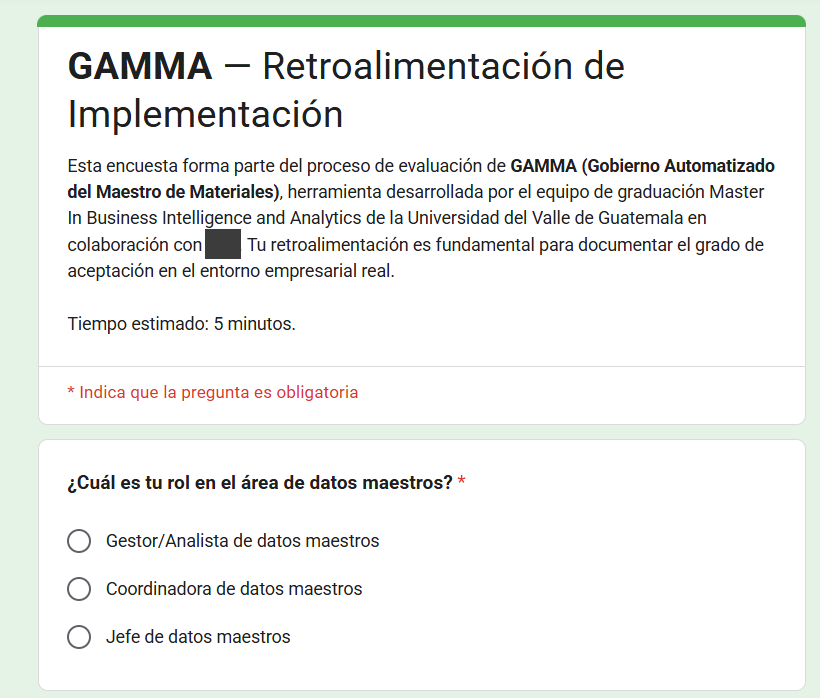
\includegraphics[width=0.85\textwidth]{figuras/encuesta_forms/forms_01_portada.png}
\caption{Portada del formulario de encuesta}
\end{figure}

\begin{figure}[!htb]
\centering
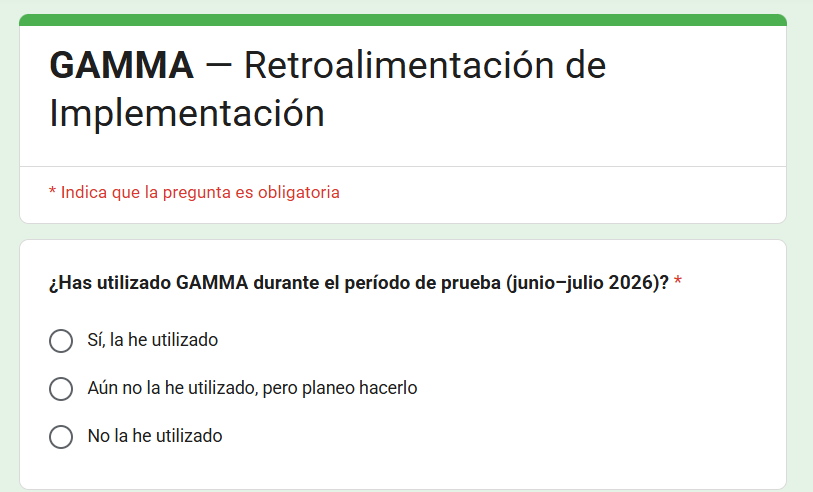
\includegraphics[width=0.85\textwidth]{figuras/encuesta_forms/forms_02_uso.png}
\caption{Pregunta de bifurcación según uso de GAMMA}
\end{figure}

\begin{figure}[!htb]
\centering
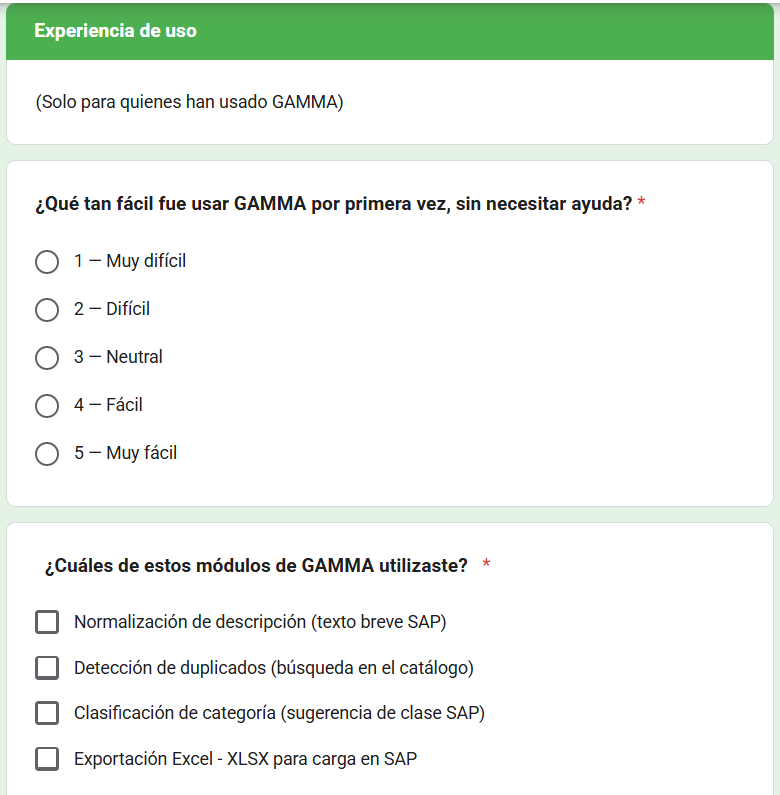
\includegraphics[width=0.85\textwidth]{figuras/encuesta_forms/forms_03_experiencia1.png}
\caption{Sección de experiencia de uso (parte 1)}
\end{figure}

\begin{figure}[!htb]
\centering
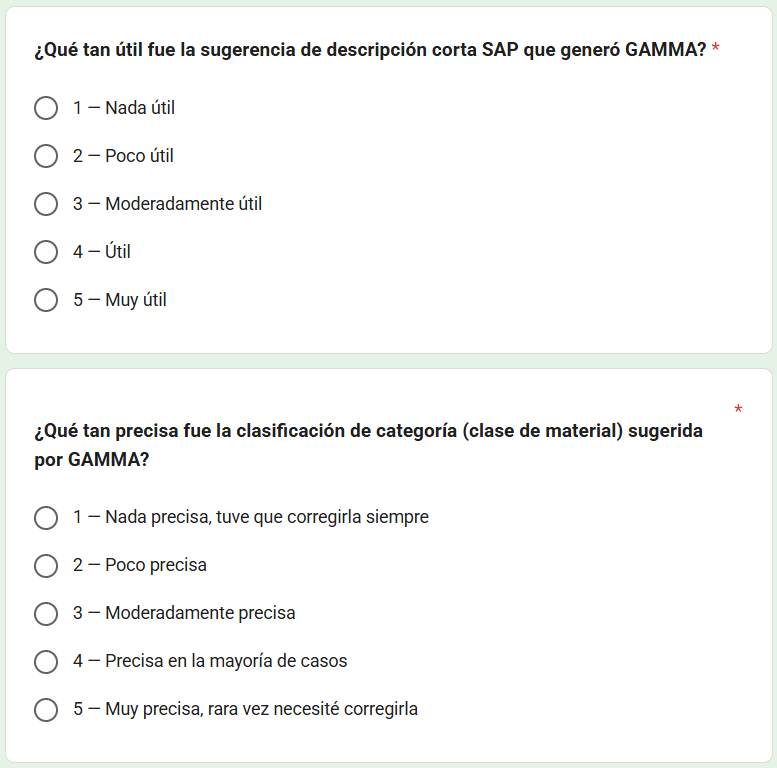
\includegraphics[width=0.85\textwidth]{figuras/encuesta_forms/forms_04_experiencia2.png}
\caption{Sección de experiencia de uso (parte 2)}
\end{figure}

\begin{figure}[!htb]
\centering
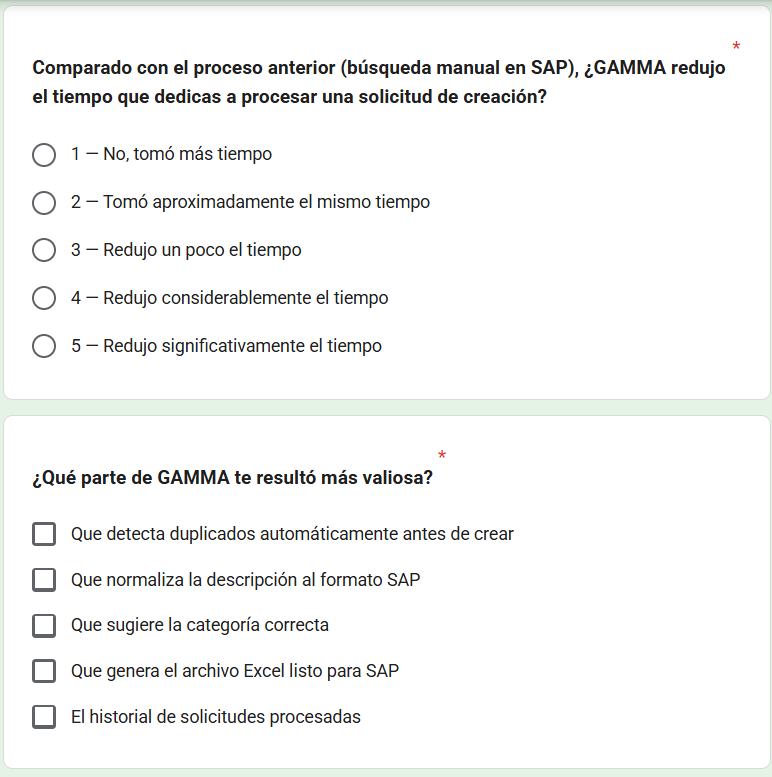
\includegraphics[width=0.85\textwidth]{figuras/encuesta_forms/forms_05_tiempo_valioso.png}
\caption{Preguntas sobre reducción de tiempo y valor percibido}
\end{figure}

\begin{figure}[!htb]
\centering
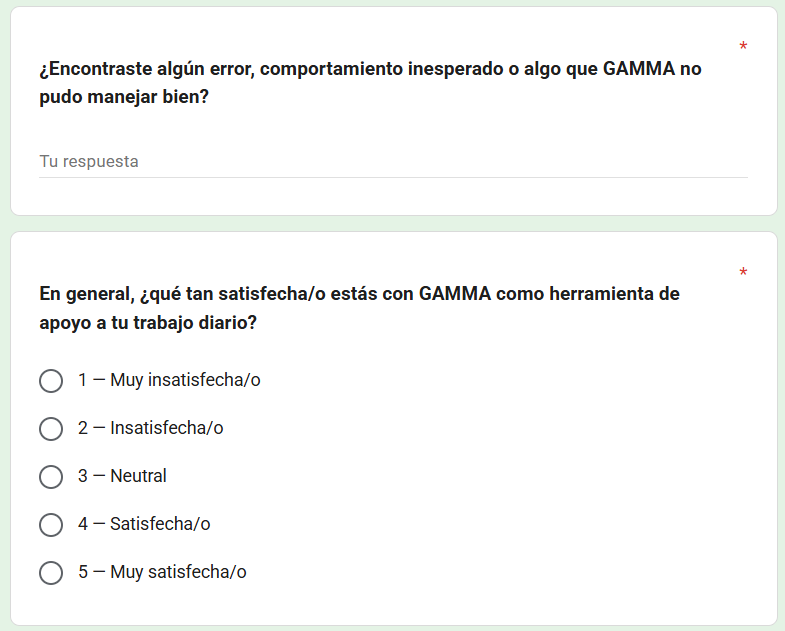
\includegraphics[width=0.85\textwidth]{figuras/encuesta_forms/forms_06_satisfaccion.png}
\caption{Preguntas de errores encontrados y satisfacción general}
\end{figure}

\begin{figure}[!htb]
\centering
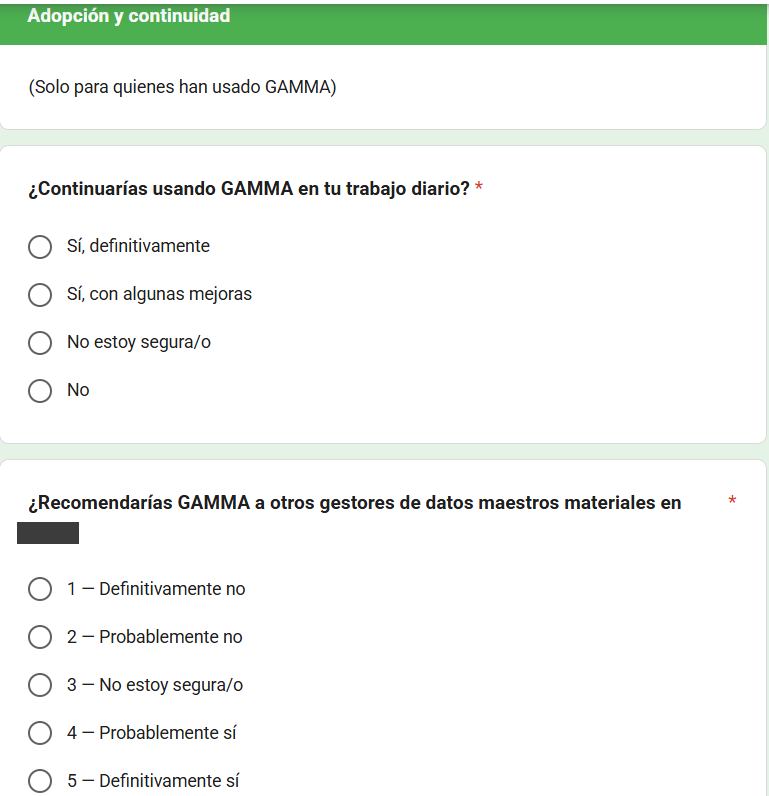
\includegraphics[width=0.85\textwidth]{figuras/encuesta_forms/forms_07_adopcion.png}
\caption{Sección de adopción y continuidad (información sensible cubierta)}
\end{figure}

\begin{figure}[!htb]
\centering

\includegraphics[width=0.85\textwidth]{figuras/encuesta_forms/forms_08_mejoras.png}
\caption{Pregunta abierta de mejoras}
\end{figure}

\begin{figure}[!htb]
\centering
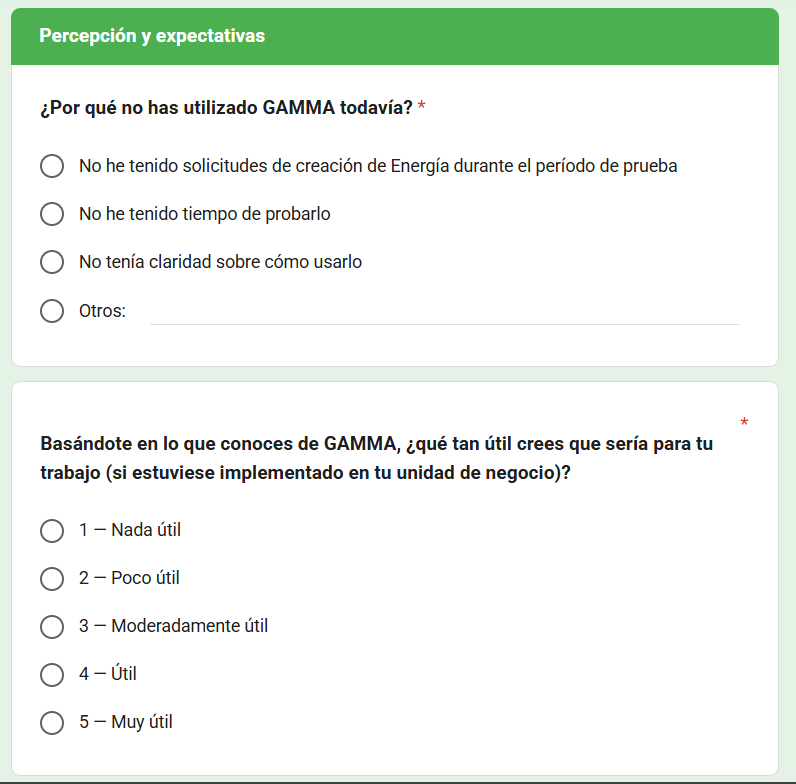
\includegraphics[width=0.85\textwidth]{figuras/encuesta_forms/forms_09_percepcion.png}
\caption{Sección de percepción y expectativas para no usuarios}
\end{figure}

\begin{figure}[!htb]
\centering
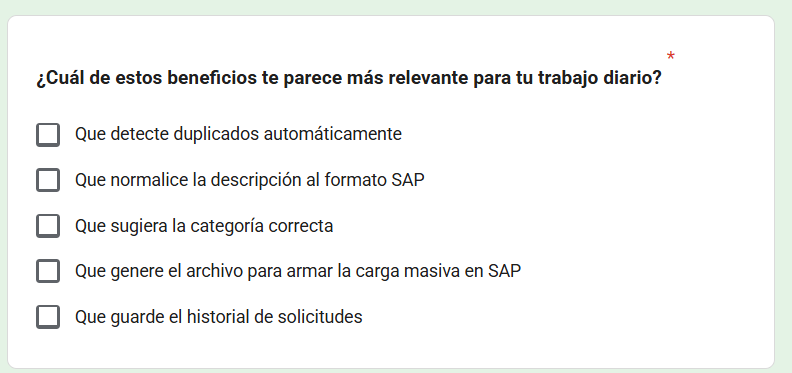
\includegraphics[width=0.85\textwidth]{figuras/encuesta_forms/forms_10_beneficios.png}
\caption{Pregunta de beneficios percibidos por no usuarios}
\end{figure}

\begin{figure}[!htb]
\centering
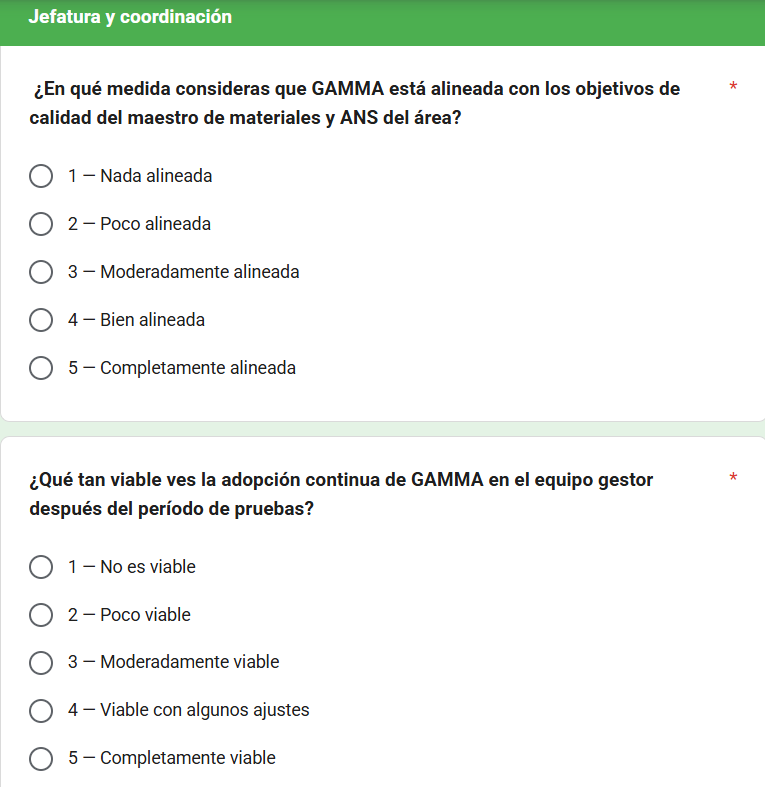
\includegraphics[width=0.85\textwidth]{figuras/encuesta_forms/forms_11_jefatura.png}
\caption{Sección dirigida a jefatura y coordinación}
\end{figure}

\begin{figure}[!htb]
\centering
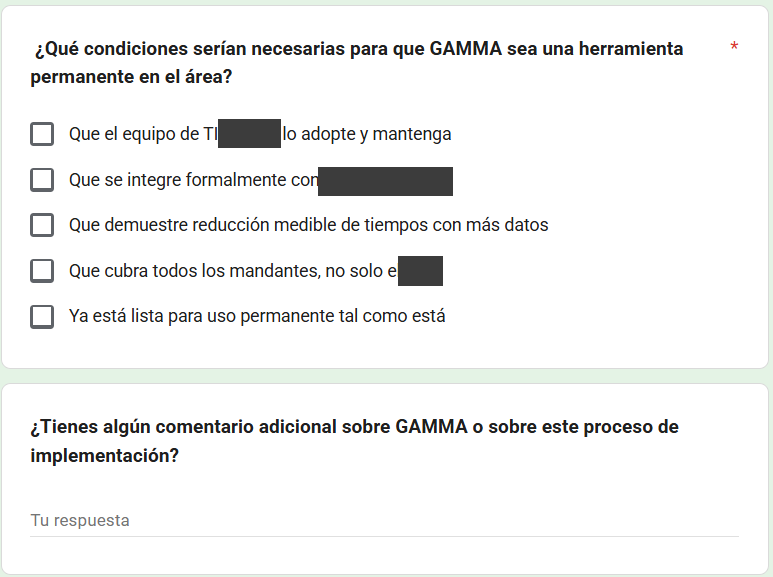
\includegraphics[width=0.85\textwidth]{figuras/encuesta_forms/forms_12_condiciones.png}
\caption{Condiciones para permanencia y comentarios adicionales (información sensible cubierta)}
\end{figure}

\chapter{Descriptor del sistema y accesos para revisión}

Este anexo describe la plataforma desplegada y las credenciales dispuestas para que el tribunal examinador pueda acceder a ella y verificar de forma directa los resultados reportados en este trabajo.

\section*{Descripción del sistema}

GAMMA es una aplicación web de página única que asiste al gestor durante la creación individual de materiales en SAP. Se despliega mediante contenedores orquestados con Docker Compose sobre un servidor privado virtual, en cuatro servicios: el motor de base de datos PostgreSQL con la extensión de similitud por trigramas habilitada; el API desarrollado en FastAPI, que concentra la lógica de negocio, la autenticación y la inferencia del modelo de clasificación; el entorno de experimentación analítica en Jupyter Lab; y el frontend, que además actúa como proxy inverso hacia los demás servicios.

La interacción principal ocurre en una interfaz conversacional. El gestor describe el material en lenguaje natural y el sistema encadena los tres módulos analíticos: normaliza la descripción a la convención de nomenclatura del catálogo mediante un modelo de lenguaje, busca coincidencias en el maestro consolidado por similitud de trigramas, y sugiere las tres categorías más probables acompañadas de su nivel de confianza. Ninguna sugerencia se registra sin confirmación explícita del gestor.

\section*{Perfiles de acceso}

La plataforma distingue dos perfiles. El Cuadro \ref{tab:accesos-modulos} resume las secciones habilitadas para cada uno.

\begin{table}[!htb]
\centering
\small
\caption{Secciones de la plataforma habilitadas según el perfil de acceso}
\label{tab:accesos-modulos}
\begin{tabular}{lcc}
\toprule
\textbf{Sección} & \textbf{Gestor} & \textbf{Administrador} \\
\midrule
Asistente conversacional (flujo de creación) & Sí & Sí \\
Tablero de indicadores & Sí & Sí \\
Ayuda y documentación de uso & Sí & Sí \\
\midrule
Arquitectura de la solución & --- & Sí \\
Referencia técnica (API y esquema de datos) & --- & Sí \\
Modelo (operación, arquitectura y evaluación) & --- & Sí \\
Entorno de experimentación analítica & --- & Sí \\
Administración de cuentas & --- & Sí \\
\bottomrule
\end{tabular}
\end{table}

El perfil de \textbf{gestor} corresponde al usuario operativo y reproduce la experiencia del equipo durante el período de validación. El perfil de \textbf{administrador} añade la documentación técnica, el detalle de la evaluación del modelo, el historial de versiones y la capacidad de ejecutar un reentrenamiento.

\section*{Credenciales de revisión}

Las cuentas del Cuadro \ref{tab:credenciales} se crearon exclusivamente para la revisión de este trabajo y son independientes de las cuentas de la operación. No permiten consultar información identificable de los usuarios del período de validación.

\begin{table}[!htb]
\centering
\small
\caption{Credenciales dispuestas para el tribunal examinador}
\label{tab:credenciales}
\begin{tabular}{lll}
\toprule
\textbf{Perfil} & \textbf{Usuario} & \textbf{Contraseña} \\
\midrule
Gestor          & \texttt{revisor.gestor@gamma.gt} & \texttt{[Jfe4b66cN2]} \\
Administrador   & \texttt{revisor.admin@gamma.gt}  & \texttt{[n8PR1JH47e]} \\
\bottomrule
\end{tabular}
\end{table}

\noindent\textbf{Dirección de acceso:} \texttt{[http://gamma.cookielab.cc]}

\section*{Instrucciones de conexión}

\begin{enumerate}
	\item Abrir la dirección de acceso en un navegador de escritorio actualizado. La aplicación no requiere instalación ni complementos.
	\item Iniciar sesión con una de las cuentas del Cuadro \ref{tab:credenciales}.
	\item La sesión permanece activa mediante un testigo de autenticación almacenado en el navegador. Para alternar entre ambos perfiles debe cerrarse la sesión desde el menú de usuario antes de ingresar con la otra cuenta.
\end{enumerate}

\section*{Recorrido sugerido}

Para verificar los resultados reportados se propone la siguiente secuencia.

\vspace{0.5em}
\noindent\textbf{Con el perfil de gestor:}

\begin{enumerate}
	\item Ingresar al asistente conversacional y solicitar la creación de un material describiéndolo en lenguaje natural, sin ajustarse a la convención de nomenclatura. Se observará la descripción normalizada propuesta, las coincidencias detectadas en el maestro y las tres categorías sugeridas con su nivel de confianza.
	\item Repetir el ejercicio con la descripción de un material que probablemente ya exista en el catálogo, para observar el comportamiento del módulo de detección de duplicados.
	\item Consultar el tablero de indicadores, donde se presentan los tiempos de gestión, el volumen procesado y los indicadores de calidad sobre los que se construyeron los resultados de este trabajo.
\end{enumerate}

\vspace{0.5em}
\noindent\textbf{Con el perfil de administrador:}

\begin{enumerate}
	\item Consultar la sección de Modelo, que reúne el diagrama del flujo de clasificación, la comparación de las siete configuraciones evaluadas, el análisis de umbral de confianza y el historial de versiones del artefacto.
	\item Consultar la Referencia técnica, que expone la documentación interactiva del API y el diagrama entidad-relación de los cuatro esquemas de la arquitectura medallón.
	\item Consultar la sección de Arquitectura para el detalle de los componentes y su despliegue.
\end{enumerate}

\section*{Consideraciones}

Las credenciales anteriores tienen vigencia limitada al período de revisión y evaluación de este trabajo, y serán desactivadas una vez concluido. El catálogo con el que opera la instancia corresponde a la extracción del maestro empleada durante el desarrollo, de modo que las consultas reflejan ese corte y no el estado vigente del ERP de la organización. Las solicitudes de creación generadas durante la revisión quedan registradas en la instancia pero no se transfieren a ningún sistema productivo.

\chapter{Tablero de vizualisación}

\begin{figure}[!htb]
\centering
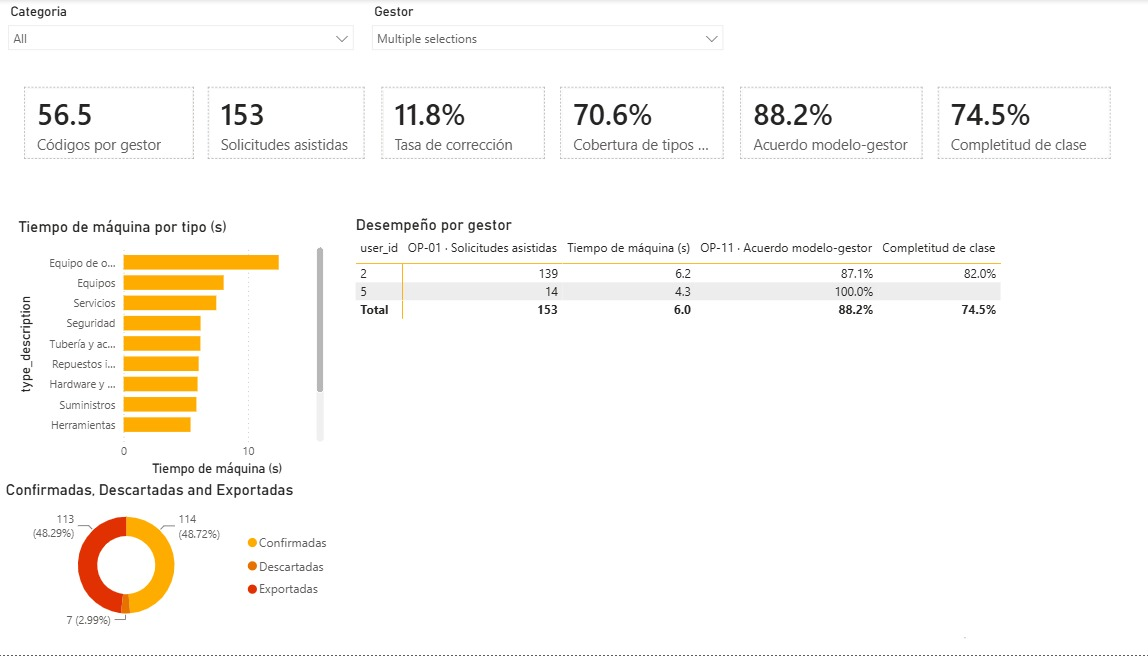
\includegraphics[width=1\textwidth]{figuras/Tablero completo.png}
\caption{Vista Inicial del Tablero Operativo}
\end{figure}

\begin{figure}[!htb]
\centering
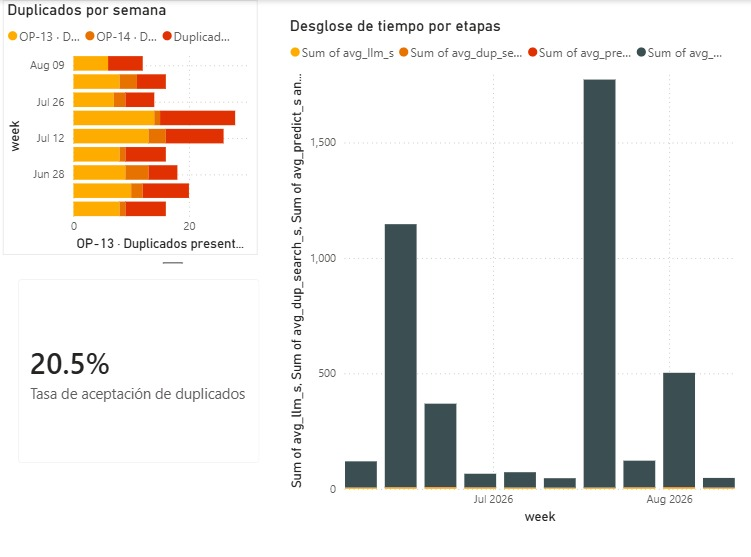
\includegraphics[width=1\textwidth]{figuras/Tablero 2.png}
\caption{Vista complementaria del Tablero Operativo}
\end{figure}